\section{L'Insee, environnement propice à la Data Science}
Ce stage a été proposé par l'Insee dans le cadre de l'une de ses mission, à savoir, celle de la diffusion de l'information statistique. Accueilli à la direction générale, j'ai eu l'occasion de découvrir le fonctionnement d'une grande administration française ainsi que son appropriation des techniques du Big Data et des Data sciences.

\subsection{Environnement professionnel}

\subsubsection{Présentation de l'Insee}
\vspace{10pt}
\begin{center}

\includegraphics[scale=0.12]{images/Logo_Insee.png} 
\end{center}

L'Institut national de la statistique et des études économiques (Insee), créé par la loi des finances du 27 avril 1946, est une administration publique rattachée au ministère de l'Économie et des Finances. Il est dirigé actuellement par Monsieur Tavernier.
\newline

L'Insee a pour mission de collecter, analyser et diffuser des informations sur l'économie et la société française sur l'ensemble de son territoire. Il organise les campagnes de recensement de la population, réalise la comptabilité nationale, mène des enquêtes sur les ménages ou les entreprises françaises, mesure les principaux indicateurs de l'économie comme le taux de chômage ou le taux de croissance. Il gère également un certain nombre de répertoires~:
\begin{enumerate}
    \item Le répertoire Sirene~: il permet d'identifier les entreprises.
    \item La base des répertoires des personnes physiques~: elle permet de certifier les états civils des individus, leur attribuer un numéro d'inscription au répertoire communément appelé «~numéro de sécurité sociale~».
    \item Le Répertoire électoral unique~: il a pour finalité la gestion du processus électoral et la fiabilisation des listes électorales.
\end{enumerate}

L'Insee est de plus en charge de nomenclatures officielles~: les Professions et Catégories Socioprofessionnelles (PCS) ainsi que le Code Officiel Géographique (COG).
\newline

L'Institut a aussi pour mission de diffuser l'information statistique à un public le plus large possible, notamment au travers de son site internet. Sont disponibles via ce portail les informations relatives à tous les services décrits précédemment. Ces informations permettent d'aider les entreprises, les particuliers, les chercheurs, les administrations et les pouvoirs publics en éclairant la situation et les enjeux économiques, démographiques et sociaux à l'échelle locale comme à l'échelle nationale. Concernant la diffusion à l'international, l'Insee contribue activement aux travaux européens portés par Eurostat, en charge de la statistique européenne officielle.
\newline

Enfin, l’Insee coordonne et anime le réseau du Service Statistique Publique (SSP) composé de services statistiques dédiés au sein des ministères (justice, travail, environnement, etc.). Elle travaille également avec d’autres organes administratifs ayant des activités statistiques (Banque de France, Ined, etc.).
\newline

L'organisation administrative de l'Insee comprend~:
\begin{enumerate}
    \item Une Direction Générale (DG) située à Montrouge (92) qui assure des tâches de conception, de coordination et d'étude au niveau national. Le centre statistique de Metz et le centre de formation de Libourne sont des entités de la direction générale implantées en région.
    \item Treize Directions Régionales (DR) en métropole et deux dans les DOM.
\end{enumerate}

\subsubsection*{La Direction du Système d'Information}

La gouvernance des sujets informatiques de l’Insee est confiée à la Direction du Système d'Information (DSI). 
\newline

Les missions de la DSI sont d’assurer la construction, les évolutions, l'exploitation et la disponibilité du système d'information de l'Insee.
\newline

La direction comporte trois entités qui pilotent respectivement les problématiques~:
\begin{enumerate}
    \item d'exploitation du SI~: Département de la Production et de l'Infrastructure Informatiques (DPII)
    \item de développement du SI~: Département du Développement du SI (DDSI)
    \item de stratégie et de cohérence du SI~: unité de l'innovation et de la stratégie du système d'information ( UnISSI), au sein de laquelle se trouve la Division innovation et instruction technique.
    \newline
\end{enumerate}

En outre plusieurs services sont déconcentrés au sein d’établissements régionaux~:
\begin{enumerate}
    \item  Le centre d’exploitation informatique (CEI) intégré au centre statistique de Metz et le service national des supports informatiques (SNSI) situé à Nantes, tous deux sous la responsabilité fonctionnelle du DPII.
    \item Quatre services nationaux de développement informatiques (SNDI) situés à Lille, Nantes, Orléans et Paris et un pôle Gestion de contenu et outils collaboratifs (PGCOC) situé à Aix-en-Provence, sous la responsabilité fonctionnelle du DDSI.
\end{enumerate}

\subsubsection{La Division Innovation et Instruction Technique}
Je suis accueilli dans la Division innovation et instruction technique (DIIT), qui comprend quatre agents. Créée en 2018, elle fait partie de l'UnISSI. La mission de la DIIT est d'offrir un cadre propice à l'innovation à l'Insee, et d'accompagner la transformation numérique de l'Institut autour de cinq grandes orientations~:
\begin{enumerate}
    \item La collaboration
    \item La statistique reproductible
    \item L'open source 
    \item La Data science
    \item Le développement d'applications orienté DataOps
    \newline
\end{enumerate}

Actuellement, la division Innovation et instruction technique assure la maîtrise d’ouvrage et la maîtrise d’œuvre de la plateforme innovation, dont une description plus détaillée est donnée section \ref{section 2.2.1}. Le maintenance de cette infrastructure s’appuie également sur du volontariat de quelques agents dans différentes entités de l’Insee. En particulier, l’intégration de certains services relève d’agents externes à la DIIT, y compris hors DSI. 
\newline

Bien que j'effectue mon travail au sein de l'équipe, mon sujet s'intégrant dans leur thématique de l'Open Source et de la Data science, il est supervisé par Franck Cotton, conseiller scientifique auprès du DSI et à l'origine du projet. 
\newline

Le SSP Lab, unité qui travaille sur l'utilisation de la Data science pour les services de statistique publiques, se montre également intéressée par mon projet. Par ailleurs ils travaillent régulièrement avec la DIIT, à l'occasion de hackaton sur la Datascience par exemple. J'ai donc l'occasion de travailler avec des personnes aux profils variés~:
\vspace{10pt}
\begin{figure}[H]
  \centering
  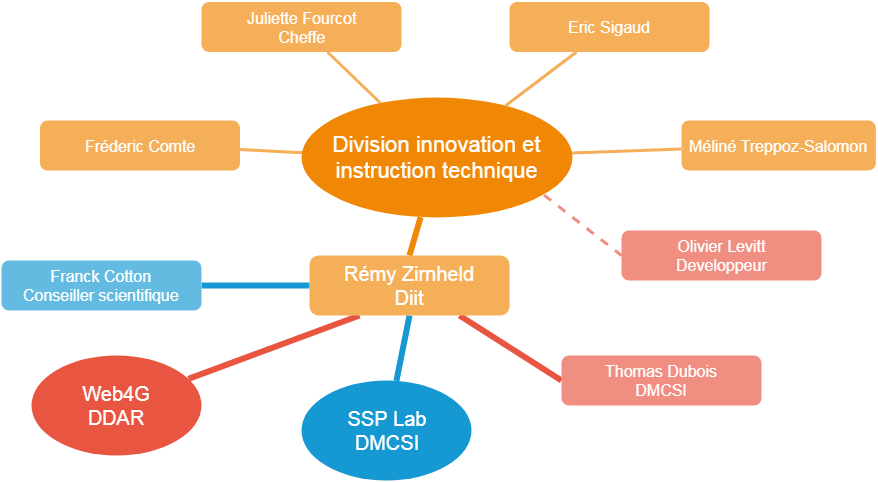
\includegraphics[scale=0.45]{images/Organigramme-stage.png}
  \caption{Liste des personnes m'aidant sur le projet}
  \label{fig:Organigramme}
\end{figure}

\vspace{20pt}

\begin{itemize}
    \item \textbf{Franck Cotton}~: Conseiller scientifique auprès de la Direction du Système d'Information. À l'origine du projet, il est le directeur du stage et me guide dans mes réflexions.
    \vspace{5pt}
    \item \textbf{Juliette Fourcot}~: Cheffe de la DIIT, elle remplace Franck pour mon suivi lors de ses nombreux déplacements. Elle m'a apporté, tout au long du stage une aide précieuse, tant sur les aspects organisationnels que techniques.
    \vspace{5pt}
    \item \textbf{Eric Sigaud}~: Membre de la DIIT, il m'apporte une aide technique sur l'utilisation de la plateforme innovation, ainsi que sur l'utilisation d'XSLT pour le traitement des fichiers XML. Il m'apporte également un oeil éclairé pour les diverses présentations que j'ai dû préparer durant ce stage.
    \vspace{5pt}
    \item \textbf{Frédéric Comte}~: Également membre de la division innovation et principal architecte de la plateforme, il m'apporte beaucoup de connaissances techniques sur la plateforme. J'ai notamment eu l'occasion de changer et configurer des nouveaux serveurs pour la plateforme.
    \vspace{5pt}
    \item \textbf{Mélinée Treppoz-Salomon}~: Membre de l'équipe innovation, elle m'aide sur l'utilisation de la plateforme ainsi que sur mes diverses présentations.
    \vspace{5pt}
    \item \textbf{Olivier Levitt}~: Développeur au Recensement de la Population (RP). Son expertise dans le développement d'application contribue au bon déroulement du projet.
    \vspace{5pt}
    \item \textbf{Thomas Dubois}~: Chef de projet statistique à l'unité qualité, incluse dans la Direction de la Méthodologie et de la Coordination Statistique et Internationale (DMCSI). Chef l'équipe en charge d'RMéS, il fournit un regard métier sur le projet.
    \vspace{5pt}
    \item \textbf{L'équipe Web4g}~: En charge du site insee.fr, l'équipe Web4g me fournit des informations sur la structure des publications, ainsi qu'un accès à la base de données qui les référence. Elle dépend fonctionnellement de la Direction de la Diffusion et de l'Action Régionale (DDAR), qui gère notamment le site de l'Insee.
    \vspace{5pt}
    \item \textbf{Le SSP Lab}~: Laboratoire du service de statistique publique. Cette équipe travaille sur les nouvelles méthodes (Datasciences et Big Data), et suit les avancées de mon projet.
    \newline
\end{itemize}

Si ce projet est réalisé par moi-même sur le plan technique, je suis accompagné dans ma démarche par ces différents acteurs.
\label{section 1.1.2}

\subsection{Le cadre du projet}

\subsubsection{Le référentiel des métadonnées statistiques}
Parmi les entités nommées à reconnaître dans les publications figurent des concepts statistiques. Ces concepts sont référencés dans le Référentiel des Métadonnées Statistiques (RMéS) de l'Insee, disponible sur le site \href{http://rdf.insee.fr/sparql}{rdf.insee.fr} \cite{rdf.insee.fr} au format RDF. Les concepts y sont décris à l'aide de plusieurs champs~: libellé, libellé alternatif, le plus souvent un acronyme, définitions et notes permettent de les identifier. Les concepts statistiques sur lesquels j'ai travaillé sont au nombre de 1162. Des liens sémantiques entre concepts enrichissent également la sémantique des concepts. En voici un exemple~:
\begin{figure}[H]
    \centering
    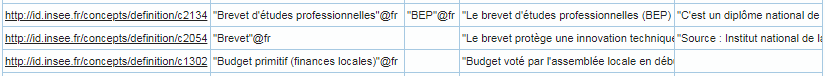
\includegraphics[scale=0.68]{images/Exemple-RMeS.png}
    \caption{Exemple de concepts de la base RMéS}
    \label{fig:exemple-rmés}
\end{figure}

Afin d'avoir une meilleure vision de ce que doit être une telle base, et à la demande de Franck, j'ai effectué une comparaison avec différentes bases de concepts au format rdf également~: 
\begin{itemize}
    \item Le thesaurus de l'\href{http://vocabularies.unesco.org/browser/thesaurus/en/?clang=fr}{Unesco} \cite{unesco}
    \item Le base de la \href{https://data.bnf.fr/current/sparql.html}{Bibliothèque nationale de France} \cite{bnf}
    \item La base de concepts d'\href{https://pro.europeana.eu/page/linked-open-data}{Europeana} \cite{europeana-rdf}
    \newline
\end{itemize}

Plusieurs particularités sont à noter~: tout d'abord, les concepts statistiques ont des libellés et définitions de tailles variées, contrairement aux autres thesaurus où les définitions sont courtes et où la taille des libellés est homogène. Cette spécificité viens du fait que les contenus sont rédigés par les responsables métier du domaine dans lequel ils sont mobilisés. Certaines informations contenu dans les libellés devraient être traduites sous la forme de triplet RDF~: «~Accueils de scoutisme (mineurs)~», «~Administrations publiques locales (comptabilité nationale)~» sont des exemples. Les définitions sont globalement plus longues et plus riches que dans les autre thesauri.

De plus, les liens entre les concepts sont nombreux, mais peu variés dans le référentiel de l'Insee, là où ils sont plus rare mais aussi plus variés dans les thesauri de la BnF et d'Europeana. Globalement, la base n'est pas hiérarchisée et les concepts apparaissent «~à plat~».
\newline

À la demande de mon tuteur, j'effectue quelques tentatives pour hiérarchiser la base. Une base hiérarchisée pourrait en effet faciliter la reconnaissance d'entités nommées, en faisant une exploration de graphe à partir des concepts dont on trouve le libellé exact dans la publication par exemple. Cela est également l'occasion pour moi de découvrir l'un des outils utilisés dans le traitement du langage naturel~: \href{https://spacy.io/}{SpaCy} \cite{spacy2}.
\label{section 1.2.1}

\subsubsection*{Premières tentatives}
La bibliothèque SpaCy propose une méthode de calcul de distance entre deux textes. Cette méthodes est basée sur le \href{https://en.wikipedia.org/wiki/Word_embedding}{\textit{Word Embedding}} \cite{word-embedding} \cite{word-embedding-opencls}, c'est-à-dire la vectorisation de mots pour en représenter la sémantique. Trois cent mille vecteurs représentant des mots assez courant de la langue française sont proposés par la bibliothèque. Ils représentent les mots dans un sens assez large~: les mots «~chat~» et «~chien~» ont par exemple des vecteurs proches, car l'on retrouve ces mots dans des contextes assez similaires. Davantage d'informations.
\newline

La tentative de hiérarchisation de la base consiste à utiliser cet outil sur les paires de concepts, pour obtenir une distance sémantique entre les deux concepts. On peut par exemple imaginer que, si l'on soumet les définitions des concepts «~Salaire~» et «~Salaire médian~» d'une part, et celles de «~Salaire~» et de «~Commerce de gros~» d'autre part, la première distance renvoyée sera normalement plus faible que la deuxième. Un rapide test me montre que c'est effectivement le cas. L'idée pour hiérarchiser la base est donc la suivante~: il s'agit d'appliquer un algorithme de \textit{Clustering} sur les concepts en utilisant la distance fournie par l'outil \textit{Similarity} de \textit{SpaCy}. Une définition de \textit{Clustering} est donnée en annexe page \pageref{clustering}. Après exécution de l'algorithme de \textit{Clustering}, on prend pour représentant de chaque cluster le concept du cluster étant le plus proche du barycentre du cluster. Ce barycentre est bien entendu pondéré par la distance sémantique des concepts.
\newline

Les premiers tests sont réalisés en fixant un seul paramètre de l'algorithme de clustering, appelé hyperparamètre~: le nombre de clusters à 100. J'ai établi cette valeur car beaucoup de concepts sur les 1162 sont censés être seuls dans leur cluster. Les principaux regroupements attendus sont ceux autour de concepts très généraux, comme par exemple le «~Salaire~», le «~Commerce~», ou encore la «~Commune~». Tous ces concepts ont en effet beaucoup de variantes plus spécifiques (entre cinq et dix) et l'on s'attend à ce qu'ils soient dans les même clusters.
\newline

Les résultats sont peu probants~: en effet, quelle que soit l'implémentation (méthode d'agrégation de clusters notamment) et les hyperparamètres utilisés, on obtient toujours le même schéma de clusters, à savoir un ou deux grand cluster rassemblant entre 100 et 200 concepts, quelques clusters de taille moyenne (2-10 concepts) et quelques clusters contenant des concepts isolés. Globalement, on retrouve bien les groupements attendus~: les concepts relatifs au salaire sont tous dans le même cluster, de même que les entités géographiques ainsi que pour les concepts relatifs au commerce. L'inconvénient est qu'ils sont en général accompagnés par d'autres concepts, excepté pour les entités géographiques qui sont seules dans leur cluster. Voici quelques exemples de regroupements~:
\newline

% TODO : mettre des exemples.

Ces résultats sont principalement dus à la méthode de calcul de distance entre deux concepts. L'outil \textit{Similarity} de \textbf{SpaCy} réalise en effet une simple moyenne des vecteurs de chacun des mots du texte, puis utilise le vecteur résultant comme représentant du sens du texte. De même que l'on peut avoir deux séries de nombres complètement différents ayant le même moyenne, on peut ici avoir deux textes complètement différents ayant le même vecteur. C'est pourquoi certains regroupement ne sont pas pertinents.

De plus, on remarque que, plus la définition est longue, plus un concept est susceptible de se retrouver dans un grand cluster. Cela est dû au fait que le calcul du vecteur représentant un texte effectue la moyenne sur tout les mots du texte. Il prend donc en compte des mots très communs, que l'on retrouve dans toute les définitions (le verbe être par exemple). Cela explique le fait que les vecteurs moyennes de longs textes se rapprochent assez naturellement. Des explications plus détaillées sur l'effet de normalisation sont fournis en annexe page \pageref{hierarchisation}. L'outil \textit{Similarity} semble finalement être adapté à une granularité assez fine~: mot, groupe de mots, et peut-être courtes phrases.
\newline

Le but principal du stage n'est pas d'améliorer la base RMéS. C'est pourquoi je ne creuse pas davantage le sujet, afin de me concentrer sur les publications et leurs traitements.
\label{section 1.2.1 - Premières tentatives}

\subsubsection{Les publications du site insee.fr}

L'objectif principal du projet est d'améliorer la qualité des publications de l'Insee. Ces publications sont diffusées sur le site \href{https://insee.fr/fr/accueil}{insee.fr} \cite{insee.fr}, récemment rénové et aujourd'hui maintenu par l'équipe Web4G.
\newline

\begin{figure}[H]
    \centering
    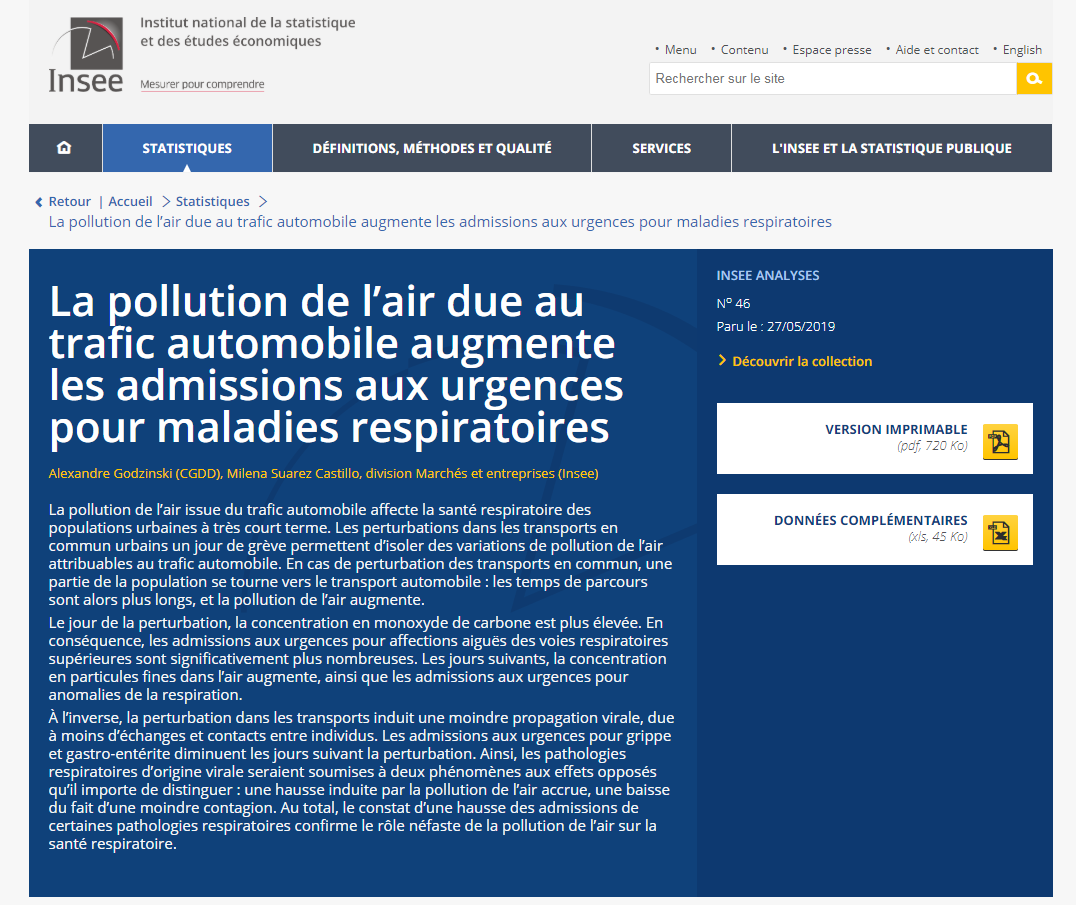
\includegraphics[scale=0.52]{images/insee-fr-exemple.png}
    \caption{Exemple de publication sur le site insee.fr}
    \label{fig:insee.fr}
\end{figure}

Les informations diffusées ont des formats divers~: tableaux, graphiques, cartes et fichiers détails accompagnent généralement les données textuelles des publications. Bien que le fichier structurant la publication soit toujours un fichier XML, le format des données textuelles est varié. Certains types de publications sont au format PDF texte, PDF image, PNG ou encore XLS lorsqu'il s'agit de tableaux. La plupart des publications où l'on retrouve du texte explicatif, du langage naturel, est présente en base de donnée sous format XML ; les différentes figures étant parfois traduites dans ce même format. Il sera donc aisé de sélectionner un corpus représentatif des publications. 
\newline

Voici un exemple de publication au format XML~: 

\begin{lstlisting}[language=XML, basicstyle=\small]
<?xml version="1.0" encoding="UTF-8" standalone="yes"?>
<publication-sans-sommaire afficher-sommaire="true"
                        afficher-sommaire-documentation="false">
	<titre>La pollution de l'air due au trafic automobile augmente 
	les admissions aux urgences pour maladies respiratoires</titre>
	<auteur>Alexandre Godzinski (CGDD), Milena Suarez Castillo, 
	division Marchés et entreprises (Insee)</auteur>
	<numero>46</numero>
	<chapo>
		<paragraphe>La pollution de l'air issue du trafic automobile [...]<paragraphe>
		<paragraphe>Le jour de la perturbation, la concentration [...]</paragraphe>
	</chapo>
	...
\end{lstlisting}

Un exemple complet est donné en annexe page \pageref{publication-xml}.
\newline

Certaines collections sont destinées à un public éclairé, comme les documents de travail ou la collection «~Economie et Statistique~», et le langage utilisé y est assez technique et parfois très spécifique. Dans la plupart des publications, un langage grand public est utilisé, avec toutefois le vocabulaire de la statistique, qui est celui qui nous intéresse ici. Les publications contiennent parfois des liens hypertextes vers les définitions des concepts statistiques mentionnées. Ces concepts sont dans leur entièreté nommés par leur libelles exactes. Dans les cas ou ils ne contiennent pas de liens, le libellé est parfois incomplet ou enrichi par des adjectifs placés au milieu du libellé, rendant la reconnaissance plus ardue. Il y a quelques fois une ambiguïté sur le concept nommé, notamment pour ceux ayant des spécificités. Voilà quelques exemples de phrases faisant mention de certains concepts~:
\begin{itemize}
    \item «~En 2018, l'activité des \textbf{secteurs commerciaux} est contrastée. Dans le \textbf{commerce de gros}, les ventes restent toniques (+ 1,9 \% en volume comme en 2017), en particulier dans le \textbf{commerce de biens d'équipement et de biens domestiques}.~», Insee Première n 1759, 21/06/2019.
    Commerce - Commerce de gros - Commerce.
    % TODO compléter avec deux exemples
\end{itemize}
\label{section 1.2.2}

\subsection{La Data science à l'Insee}

L'Insee jouit d'une situation particulière dans le domaine du \textit{Big Data} et des \textit{Data sciences}. Tout d'abord, en tant qu'institut d'envergure nationale, il dispose d'une culture du traitement de la donnée, et par conséquent d'une solide expérience sur les problématiques de qualité des données brutes. Cela est en effet l'une des étapes prenant le plus de temps dans les Data sciences~: la préparation des données.
\newline

L'institut dispose par ailleurs d'une légitimité et d'un droit d'exploitation des gisements de données de par son activité. Le Règlement Général sur la Protection des Données a contraint les entreprises à trouver d'autres moyens d'obtenir des données. Cela se traduit souvent par la génération en interne de données, parfois difficile.
\newline
% TODO : compléter avec les références juridiques, étoffer

L'Insee dispose enfin de compétences de haut niveau dans le domaine des statistiques, domaine connexe à celui de la Data science. J'ai d'ailleurs pu obtenir des aides précieuses, notamment dans l'explication des concepts ou encore dans l'utilisation de certains algorithmes.
\newline

\subsection*{Conclusion}
L'environnement que j'ai découvert et l'étude des données sur lesquelles j'ai été amené à travailler m'ont permis de mieux formaliser les rendus du stage.

L'objectif est de construire un premier service de reconnaissance d'entités nommées qui se focalise sur les concepts statistiques de la base RMéS dans les publications de l'Insee. Il s'agit également de fournir de la documentation sur le traitement du langage naturel et les principaux outils existants aujourd'hui.
